\chapter{Estrategias de inversión}

\section{Plan de inversión a largo plazo}

Vamos ha estudiar un ejemplo sobre qué activo vamos a trabajar y cómo podríamos hacer este plan de inversión a largo plazo, y cuáles serían las características de este plan de inversión.

El \ti{supuesto básico} es que \tb{la inversión en bolsa en el largo plazo es siempre rentable}, aquí volvemos a un gráfico que ya vimos sobre la evolución de uno de los principales índices que es el \ti{Dow Jones}.

\begin{center}
    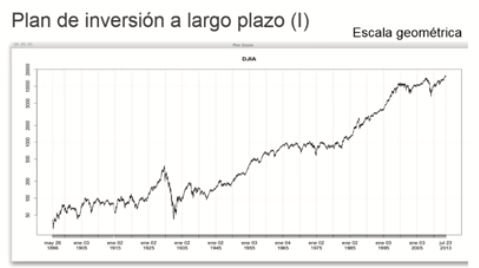
\includegraphics[scale=.85]{images/mod03-01.png}
\end{center}

El gráfico abarca del año 1896 hasta la fecha actual, donde se ve que la inversión en bolsa acaba siendo rentable en el largo plazo.

Apoyándonos en el gráfico podemos señalar:
\begin{itemize}
    \item Si no se eleige el momento de entrada adecuado, puede que tengamos que soportar, durante períodos largos, caídas muy importantes de nuestro capital invertido. Si alguien invirtió a principios de 1929 abría soportado una caída bursátil del \ti{90\%}.
    \item No es bueno invertir todo nuestro capital en un mismo instante de tiempo, lo que proponemos es \tb{periodificar la inversión} durante un período de tiempo, que cuanto más largo sea mejor ratio \ti{rentabilidad-riesgo} nos va a proporcionar.
    \item Introduciremos una nueva medida de riesgo. Vimos que generalmente la medida de riesgo utilizada es la \ti{desviación típica de los rendimientos}; sin embargo, ésta tiene como desventaja que viene medida en un tipo de unidad difícil de entender para el inversor medio o común. Vamos a introducir una nueva medida de riesgo que se conoce como \tb{drawdown}, mide la caída en terminos porcentuales desde un máximo hasta un mínimo entre dos puntos. En el caso expuesto de la caída del $90\%$, si analizamos la rentabilidad obtenida en el largo plazo, y suponemos que realizamos una inversión y que da una rentabilidad del $500\%$, la caída podría representar un $20\%$ dentro de toda esa rentabilidad obtenida. Es decir, para medir el \tb{drawdown} mediremos \ti{la caída en términos porcentuales respecto de la rentabilidad total que se espera obtener de la inversión}.
\end{itemize}

Nos centraremos en el índice Dow Jones, si analizamos su rentabilidad, tenemos el siguiente histograma de rentabilidades anuales para todo el período considerado,
\begin{center}
    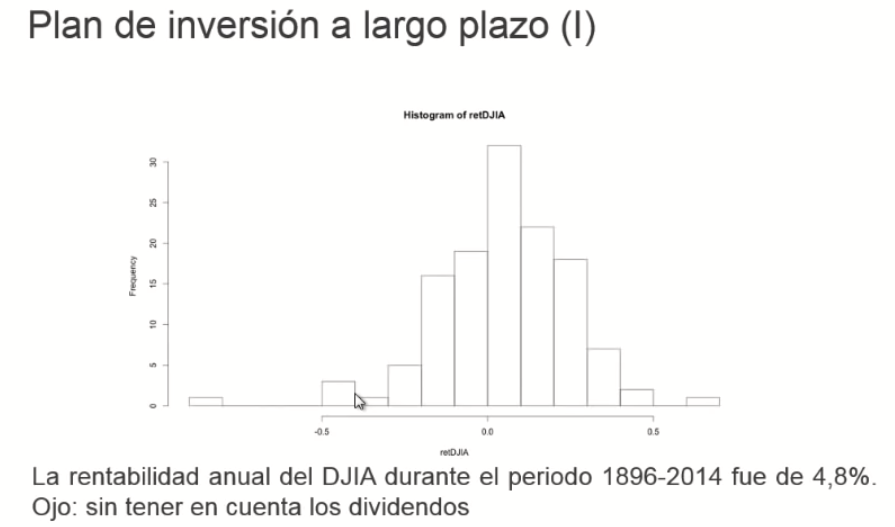
\includegraphics[scale=.65]{images/mod03-02.png}
\end{center}
la rentabilidad anual media ha sido del $4,8\%$, sería la rentabilidad mínima que los inversores deberían haber peido a cualquier inversor bursátil, eso sin tener en cuenta los dividendos, que hemos visto que durante gran parte de la historia han estado por encima del $3\%, 4\% o 5\%$, esa rentabilidad debería añadirse al $4,8\%$.

Si nos centramos, no en todo el período histórico, si no en la franja que va desde 1932, después de la crisis del 29, hasta la actualidad, entonces la rentabilidad ha sido todavía mayor, del $6,7\%$, a lo que añadimos la rentabilidad por dividendos, como mínimo del $3\%$, es fácil ver que la rentabilidad mínima que podríamos obtener sería del $10\%$, que empieza a ser una rentabilidad interesante en el largo plazo.
\begin{center}
    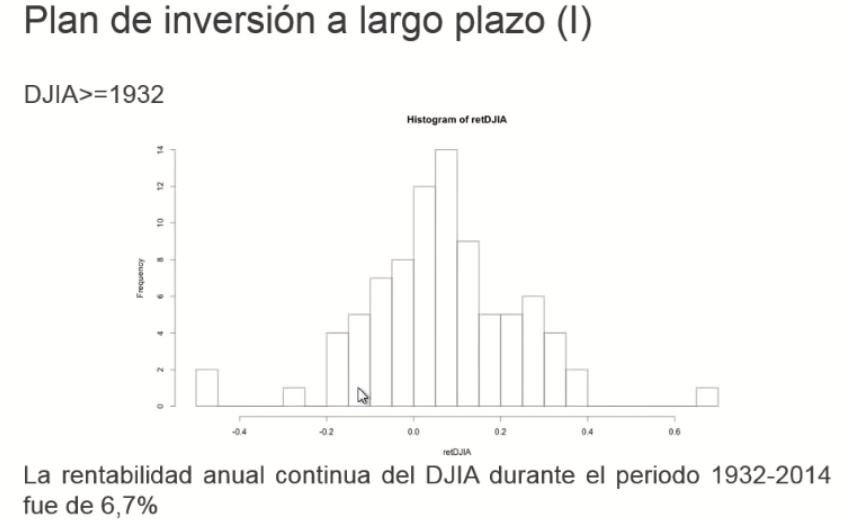
\includegraphics[scale=.65]{images/mod03-03.png}
\end{center}

Analicemos alguna otra cuestión relativa al primer gráfico sobre la evolución del Dow Jones, qué es lo que ocurre si realizamos toda nuestra inversión en un momento determinado de tiempo, si invertimos todo nuestro capital en ese instante de tiempo determinado.
\begin{center}
    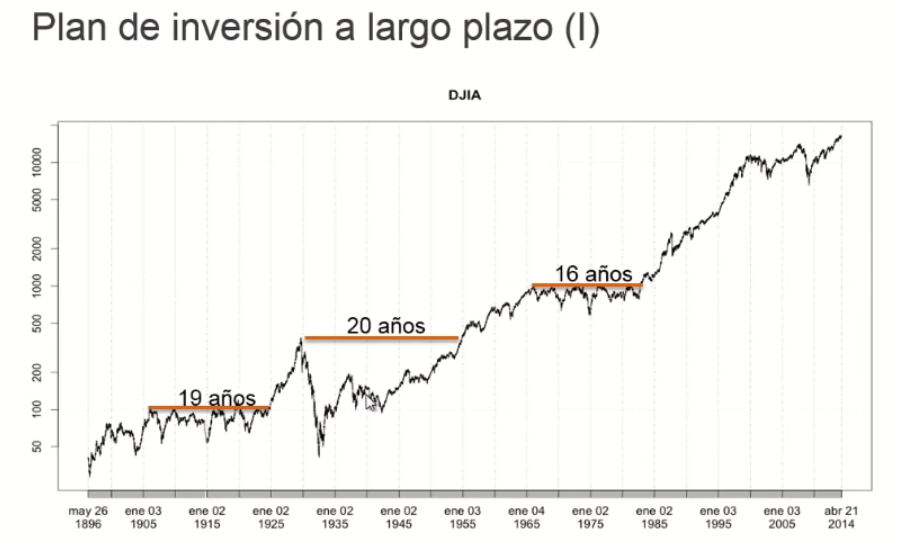
\includegraphics[scale=.65]{images/mod03-04.png}
\end{center}
Puede ocurrir que tengamos que sufrir fuertes caídas en bolsa, de las que tardaremos mucho en recuperarnos. 

Si lo que queremos hacer nuestro propio plan de inversión, y no tener que pagar, por ejemplo, las comisiones, en algunos casos demasidado altas, de los fondos de inversión, es posible que la variable más importante que tenga que ver es cuánto tiempo voy a requerir para recuperarme de alguna de estas caídas.

En la gráfica se nos muestran tres tramos o períodos:
\begin{itemize}
    \item El primero que abarca 19 años, quienes invirtieron al comienzo del mismo, durante ese tiempo tuvieron constantes vaivenes, donde no era ni alcista ni bajista y no pudieron obtener rentabilidad alguna en su inversión. Esto es algo que debemos evitar. Por lo tanto en este tramo no sería la mejor opción invertir el $100\%$ de nuestro capital, deberíamos seguir otra estrategía.
    \item El segúndo tramo está referido a la caída del 29. Quien invirtió en máximos, previos a la caída, tuvo que esperar 20 años para recuperar la inversión, siendo todavía peor que el anterior, ya que soportó una caída del $90\%$.
    \item En el tercer tramo es similar al primero.
\end{itemize}

En conclusión, 
\begin{itemize}
    \item si la inversión se produce en un único instante de tiempo se corre el riesgo de no recuperarla hasta pasado mucho tiempo, tenemos que intentar evitarlo.
    \item el riesgo no se medirá como la \ti{desviación típica} de los rendimientos, sino que utilizaremos una medida que sea más comprensible, el \ti{drawdown}, la caída de máximos en términos porcentuales.
\end{itemize} 

Para evitar estas situaciones:
\begin{enumerate}
    \item La \tb{periodificación de la inversión}, no invertir todo el capital en un único instante de tiempo, si queremos mantener la inversión durante 20 años, repartiremos la inversión durante los 20 años.
    \item La estrategia que seguiremos es invertir una misma cantidad, puede ser de \euros{1.000} o \euros{10.000}, dependerá del capital que cada uno disponga, cada seis meses. Supongamos que $X = 1$ y que dicha cantidad aumenta un $1\%$, incremento que denominamos como \tfun{g}, cada 6 meses.
    
    Eso significa que si invierto \euros{1.000}, dentro de 6 meses tendré que invertir \euros{1.000}+$1\%$ = \euros{1.010}, dentro de 12 meses sería $\euros{1.000}\ast (1,01)^2$, cada seis meses incrementaría esa cantidad en el $1\%$, de tal maner que  si la inversión se prolonga durante 20 años, la última cantidad invertida asciende a $1\ast(1+0,01)^{39} = 1,47$, si invierto inicialmente \euros{1.000}, la última aportación a la inversión será de \euros{1.470}.
    \item Finalmente, durante ese período de tiempo ¿cuánto habré invertido?, para ello utilizamos la siguiente fórmula:
    $$S = X \ast ((1 + g)^{\text{per}}-1)/g = 1\ast ((1+0,01)^{40}-1)/0,01 = 48,886$$
    Nuestro objetivo es que al final de los 20 años, la cantidad que recuperemeos sea mayor de esos \euros{48,886}. Si queríamos obtener una rentabilidad superior al $10\%$, la cantidad final deberá ser muy superior a los \euros{48,886}.
\end{enumerate}

Hemos visto que importe tendríamos que invertir cada 6 meses durante 20 años, inversión a largo plazo. Terminariamos invirtiendo \euros{48,886}, teniendo en cuenta que \ti{X = \euros{1}}, el importe final tendríamos que multiplicarlo por la cantidad con la que queremos comenzar la inversión, si ésta es de \euros{1.000}, la inversión final sería de \euros{48.886}. Lo que queremos saber es, ¿esos \euros{48.886} en cuánto acaban convirtiéndos para poder calcular la rentabilidad?.

Veamos que rentabilidades habríamos obtenido si la inversión se hubiera realizado sobre el índice Dow Jones.

\begin{center}
    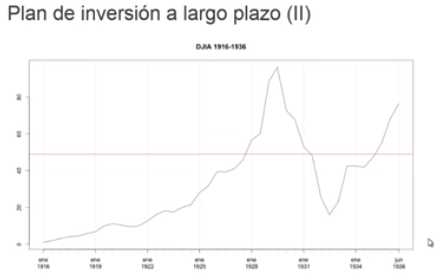
\includegraphics[scale=.65]{images/mod03-05.png}
\end{center}
En el gráfico se puede analizar la evolución durante el período 1916-1936, la primera cantidad la invertiremos en el primer semestre de 1916, y la última el último semestre de 1936. La línea roja representa la cantidad que finalmente estamos invirtiendo, los \euros{48,886}. Se observa que conforme pasa el tiempo la inversión aumenta su valor hasta un punto máximo en el que comienza una caída abrupta, que coincide con la crisis del 1929. Cuando toca fin la caída comienza una nueva recuperación, hasta el último semestre del 1936 donde se sitúa en torno a las setenta y cinco unidades.

¿Cuál habría sido la rentabilidad obtenida?. Habríamos invertido casi cincuenta unidades (\euros{48,886}) y acabamos obteniendo setenta y cinco unidades, lo que significa que estamos teniendo una rentabilidad del $50\%$ sobre la inversión realizada. El \ti{«pero»} sería que hemos sufrido la mayor crisis bursátil de la historia, lo que ha disminuido nuestro rendimiento, aún así se comprueba que no sólo se recupera lo invertido, sino que obtenemos una rentabilidad del cincuenta por ciento, uqe no está nada mal dada las circunstancias.

Tenemos que analizar que ocurre con otros períodos de veinte años. Por ejemplo, qué ocurre si iniciamos la inversión en el año 1926 y la finalizamos en el 1946,

\begin{center}
    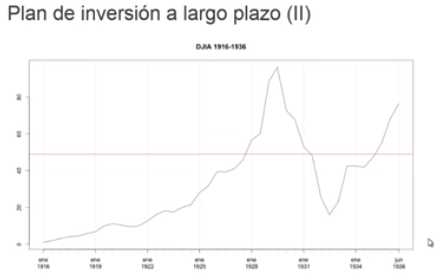
\includegraphics[scale=.65]{images/mod03-05.png}
\end{center}
Vemos que el período analizado terminaría con una rentabilidad entorno al ochenta por ciento, una rentabilidad superior a la vista del cincuenta por ciento anterior. De nuevo hemos padecido la crisis del año 29, y lo más importante, lo que tardamos en recuperarnos de esa crisis, sólo en 4 años hemos recuperado el capital, y eso debido a seguir la estrategia de la \ti{períodicidad de la inversión}.

Otro período de veinte años sería el que va de 1936 a 1956, aquí ya no le afecta directamente la crisis bursátil del 29.

\begin{center}
    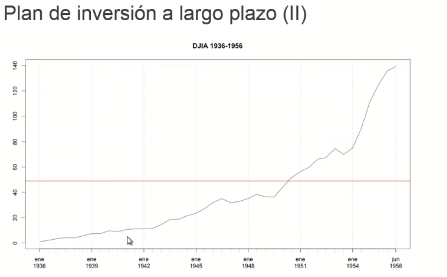
\includegraphics[scale=.65]{images/mod03-07.png}
\end{center}
Se observa como apenas hay caídas y nuestra inversión casi contínuamente hasta case ciento cuarenta unidades, prácticamente multiplicamos por tres lo invertido, estamos hablando de una rentabilidad en torno al $200\%$. 

Algo parecido ocurre con el período 1946 a 1976.

\begin{center}
    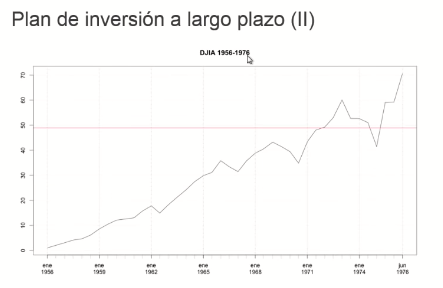
\includegraphics[scale=.65]{images/mod03-08.png}
\end{center}
Aquí la rentabilidad es menor, entorno a las setenta unidades. En sucesivos périodos tenemos más o menos los mismos resultados, y pasamos a ver la última serie, la que abarca los años 1993 a 2014.

\begin{center}
    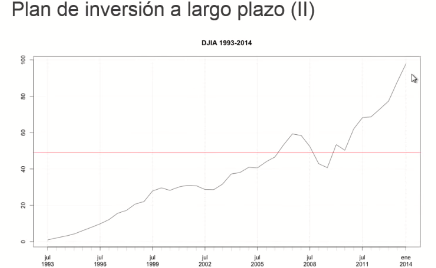
\includegraphics[scale=.65]{images/mod03-09.png}
\end{center}

Resumiendo, en ninguno de estos casos se finaliza perdiendo dinero, y por lo general, la rentabilidad mínima ronda el 50\%, siguiendo la estrategia que no requiere dedicación de tiempo, sino una estrategia  a largo plazo donde cada seis meses invertimos la misma cantidad. Esta sería la estrategia adecuada para personas cuya actividad profesional no está ligada a la bolsa, pero quieren rentabilizar su capital dedicándole un esfuerzo mínimo.

Qué ocurre si observamos la evolución de esta estrategia, empezando la inversión en el año 1916, 1917, 1918, 1919, etc. esto nos permitiría tener muchísimos más períodos de 20 años contemplados, y los resultados obtenidos serían más consistentes, no se podría decir que se deben al azar.

Esto es lo que hemos hecho, hemos observado los subperíodos de 20 años desde 1916 a 2014 para el DJIA, y su representación en un histograma sería

\begin{center}
    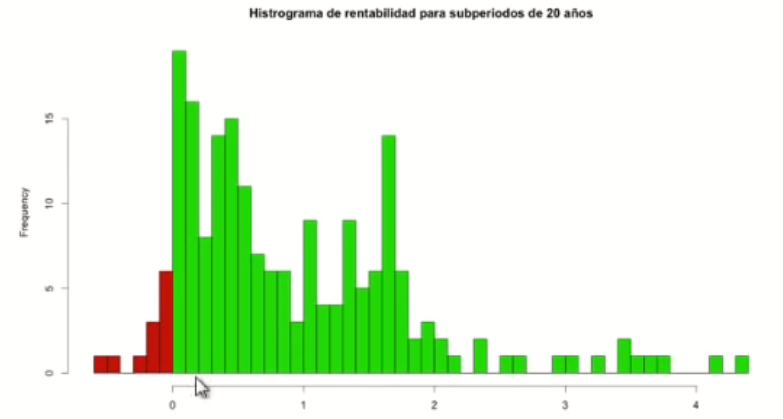
\includegraphics[scale=.65]{images/mod03-10.png}
\end{center}
En rojo están los períodos en los que se pierde rentabilidad, perdemos capital, en verde aquellos períodos en los que la rentabilidad es positiva; el 1 indica que obtenemos una rentabilidad del 100\%, el 2 del 200\% y así sucesivamente. En el histograma se observa que el 94\% de los subperíodos obtuvieron una rentabilidad positiva, sin tener en cuenta los dividendos, es decir, la probabilidad de \tb{no obtener rentabilidad del capital inicial invertido} es sólo del 6\%, el 94\% obtendremos rentabilidades positivas.

Si consideramos los dividendos, que por ejemplo tuviran una rentabilidad media del 4\% por dividendo,

\begin{center}
    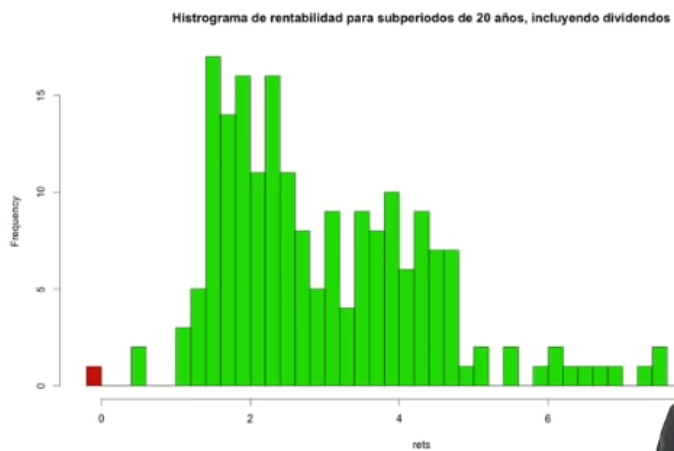
\includegraphics[scale=.65]{images/mod03-11.png}
\end{center}
Vemos que sólo un subperíodo obtiene una rentabilidad negativa, 0,5\% de los casos, la probabilidad de ganar dinero en el largo plazo sería del 99,5\%, podemos asegurar que prácticamente nuestra revalorización está asegurada y es de aproximadamente un 300\%, es decir, estaría multiplicando por 4 el capital inicial.

\section{Estrategias de trading}

Hasta ahora hemos vistos estrategias a seguir por el inversor pasivo, aquél que quiere cubrirse del efecto negativo que puede tener la inflación sobre sus ahorros, su capital. 

A continuación analizaremos posibls estrategias a utilizar por aquellos inversores que quieren hacer \tb{tradding}, algo más agresivo, no se trata del largo plazo, sino un tradding a \tb{medio plazo} o a \tb{corto plazo} e incluso \tb{intradía}.

Basaremos nuestra estrategia de inversión en la \ti{identificación y utilización de figuras técnicas, la \tb{bandera}}.

Lo que nos interesa es ver si al aplicar la estrategia sobre diferentes tipos de activos, de time frames o ventanas temporales obtenemos finalmente una rentabilidad positiva, sostenible en el largo plazo, y  si es posible con el mínimo riesgo posible.

En la actualidad, se estima que aproximadamente el 75\% de las operaciones diarias que llevan a cabo los \ti{mercados financieros} son realizadas por \ti{aplicaciones de programas}, lo que se conocen como \tb{robots}. Es decir, el \ti{tradding algorítmico} gana cada vez más peso y se basa en:
\begin{itemize}
    \item La idea de aplicar estas estrategias.
    \item Validarlas a través de algún paquete informático sobre diferentes activos y ventanas temporales, para tener la seguridad de que esa estrategia funciona y lo hace bien.
\end{itemize}

En nuestro caso bamos a desarrollar un estrategia basada en la figura conocida como \tb{flag (bandera)}. Básicamente \ti{flag} consiste en una ruptura brusca del precio que es seguido por un período en el cual el precio se mantiene con menos volatilidad, dentro de un rango determinado. Eso augura un nuevo movimiento abrupto del precio que es el que intentaremos aprovechar a través de esta estrategia.

Veamos como aplicar esta estrategia siguiendo una serie de pasos.

\begin{center}
    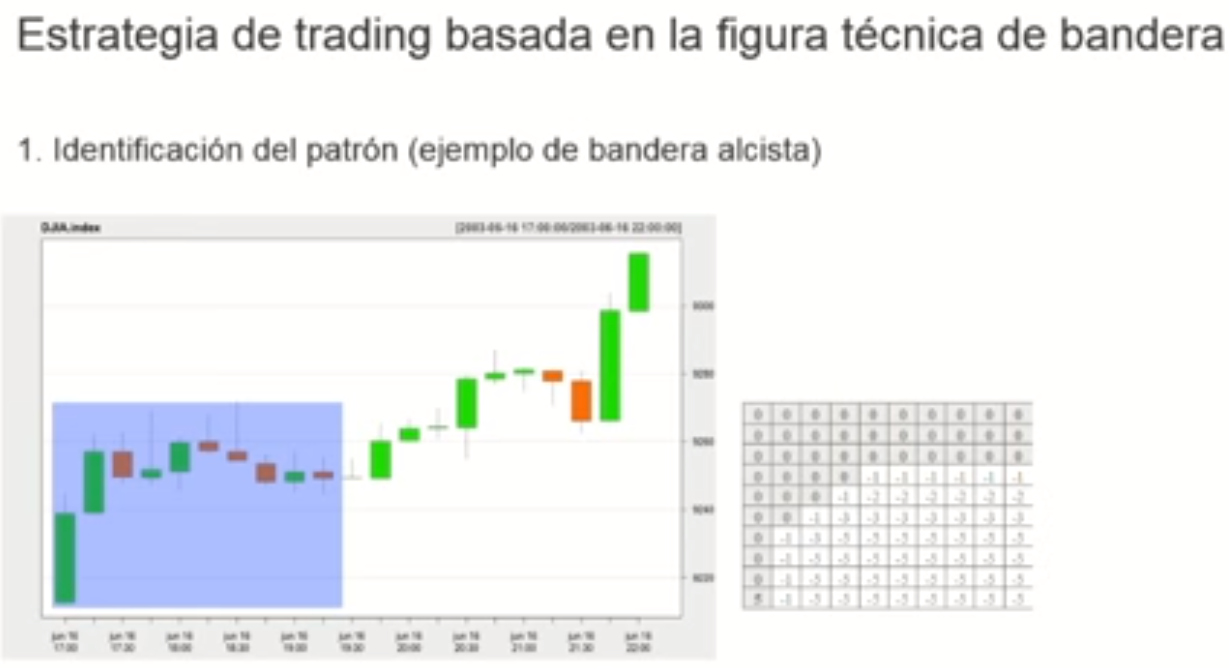
\includegraphics[scale=.45]{images/mod03-12.png}
\end{center}

\begin{enumerate}
    \item Identificar el patrón. Hemos dicho que básicamente la bandera  refleja un movimiento abrupto del precio. En el gráfico, zona sombreada, vemos que la primera bandera representa un movimiento alcista, el precio sube con fuerza, de repente se separa, se mantiene dentro de un rango determinado, con subidas y bajadas (zona sombreada), y lo que esperamos es que siga la tendencia alcista, el momento en el que el precio vuelve a romper hacia arriba. Esta zona sombreada sería la identificación del \ti{patrón bandera}, en nuestro caso sobre el índice DJIA. Además, estamos trabajando sobre datos de quince minutos, cada una de las velas se corresponde con el movimiento de precio en quince minutos.
    
    ¿Cómo identificamos las banderas?. Podemos hacerlo visualmente, pero si lo que queremos es analizar esta estructura y plantear una estrategia y aplicarla sobre una ventana temporal, hay que automatizar la identificación del patrón. En nuestro caso, lo que se hizo fue desarrollar una \ti{matriz de pesos} que se superpone sobre la ventana de precios

    \begin{center}
        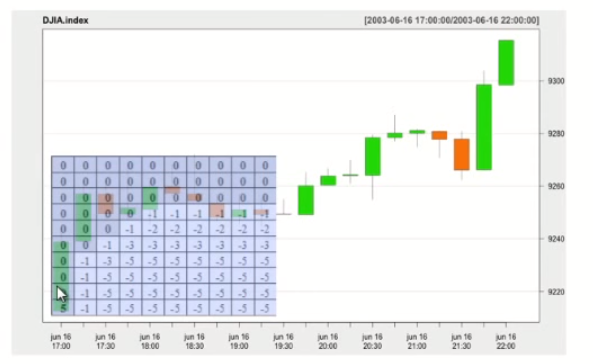
\includegraphics[scale=.65]{images/mod03-13.png}
    \end{center}
    Lo que se intenta es que los precios caígan sobre las celdas que aparecen etiquetadas como cero. Si hay algún precio que se sale de esta zona, cayera por la zona inferior de la tabla, menos sombreada, entonces no identificariamos ese movimiento con el correspondiente patrón bandera. Aquí vemos como el precio rompe hacia arriba, se mantienen las celdas que aparecen con valor 0, y hay tres celdas que aparecen con valor de -1, es decir, \ti{no sería una banderea perfecta} que puedieramos identificar de manera inequivoca, pero sí se acercaría bastante al haber sólo tres celdas que incumplen la propiedad. Seamos permisivos e identifiquemos esta situación como \ti{patrón bandera}, sería una \ti{bandera alcista}, la ruptura del precio se ha hecho hacia arriba, alcista, ha entrado en un rango en el lateral, y lo que intuimos es que el precio va a romper hacia arriba. Lo que haríamos en este caso es tomar una \ti{posición larga}, compraríamos el activo DJIA, en el punto anterior a la primera vela que sale de la matriz de pesos.

    \item Ya hemos identificado un \ti{patrón bandera}, lo que hacemos es iniciar la operación, marcando los niveles de \tb{stop loss} y de \tb{take profit}. Estos dos conceptos, básicamente ayudan a realizar una gestión monetaria correcta:
    \begin{itemize}
        \item \tb{take profit}, nos marca el nivel de beneficio que aspiramos a tener en la operación.
        \item \tb{stop loss}, marca la pérdida máxima que estamos dispuestos a asumir.
    \end{itemize}
    Si el precio evoluciona a nuestro favor cerraremos la operación una vez que el precio haya alcanzado el nivel marcado para el \ti{take profit}, si el precio va en nuestra contra, hemos comprado en largo y de repente el activo empieza a caer, cerraremos la operación en el nivel de \ti{stop loss} que hayamos marcado y, simplemente, asumiremos la pérdida.
    \begin{center}
        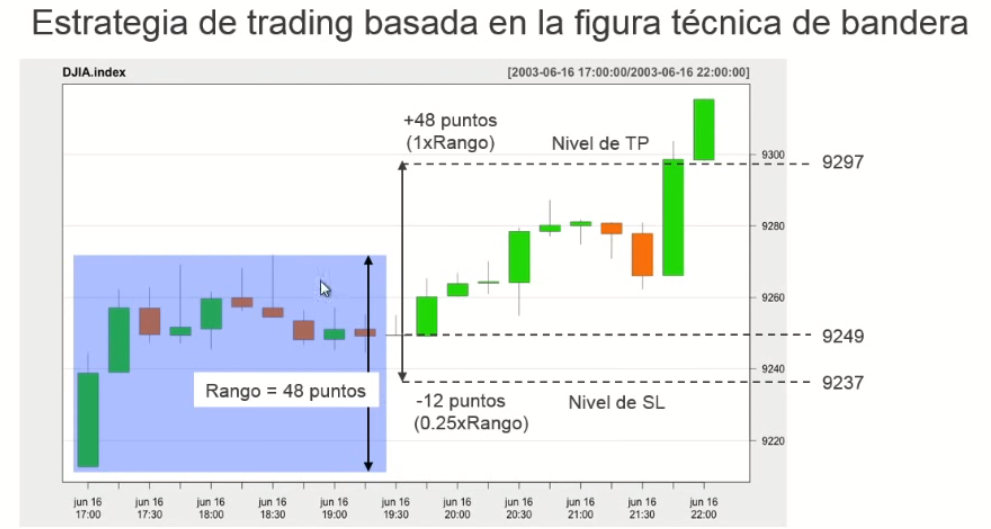
\includegraphics[scale=.65]{images/mod03-14.png}
    \end{center}
    En este caso, dentro de la ventana de 10 velas (zona sombreada gris), tuvo un rango de 48 puntos, es decir, la diferencia entre el máximo del precio y el mínimo. 

    Nosotros, lo que hacemos es marcar un \ti{take profit} que tenga ese mismo rango de puntos. Si compramos en un nivel de 9249 puntos, le sumamos 48 y esa será la cantidad de nuestro \ti{take profit} = 9297 puntos, estamos tomando como \ti{take profit} 1 por el rango (48 puntos). ¿Cuánto corresponde al \ti{stop loss}?. Hay una regla básica en el análisis técnico que nos dice que el \ti{stop loss} debería ser lo más bajo posible y siempre inferior al \ti{take profit}, es decir, si quiero una rentabilidad de 48 puntos, la máxima pérdida que esto dispuesto a soportar tiene que ser inferior a 48. En este caso hemos considerado una cuarta parte del rango (48/4 = 12), el ratio es de 4 a 1. Por lo tanto, si compramos el índice en 9249 puntos, le restariamos 12 y obtendríamos un \ti{stop less} de 9237. Si el precio baja hasta esta posición, cerramos la posición y asumimos una pérdida de 12 puntos.

    En este caso, lo que ocurrió es que el precio fué hacia arriba hasta que llegó al nivel marcado como \ti{take profit}, por lo que el beneficio de esta operación habría sido de 48 puntos. La operación se habría abierto a las 19:15 o 19:30 y la habríamos cerrado a las 21:45, se trataría de una operación \ti{intradía}.
    \item Esta estrategia debe aplicarse ahora sobre diferentes índices bursátiles como DJIAX, DAX, FTSE, IBEX y sobre diferentes pares de divisas: EUR-USD, USD-JPY, USD-CAD, USD-AUD; esto se hace para ganar consistencia, para ver que efectivamente esta estrategia de trading funciona, no sólo para un activo, sino para otros índices y diferentes pares de divisas. Se aplicará no sólo sobre velas de 15 minutos, sino también sobre velas de 1 hora, 4 horas e incluso velas diarias.
    
    Lo que necesitamos, para validar una estrategia, es el mayor número de observaciones posibles, en nuestro caso lo que hicimos fue analizar el DJIA desde el 22 de mayo del 2000 hasta el 29 de novimbre e 2013, utilizamos velas de 15 minutos, lo que supone que el trabajo de validación de estrategias se hizo sobre un total de 91.300 velas, aquí si contamos con una base de datos muy amplia y por lo tanto los resultados que se obtengan tienen validez estadística. 

    También se hicieron cambios en los valores de \ti{stop less} y de \ti{take profit} para saber exactamente con qué configuraciones la estrategia resultaba más rentable.

    \begin{center}
        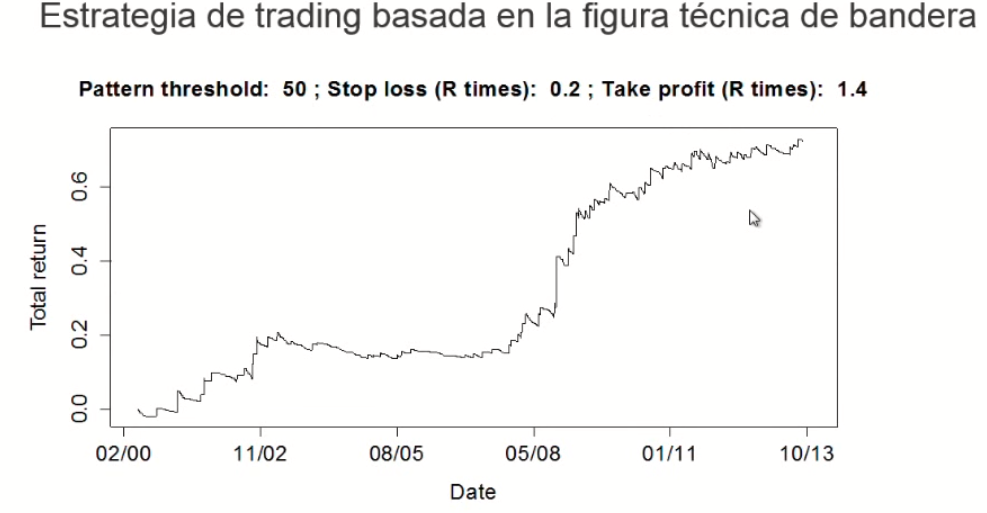
\includegraphics[scale=.65]{images/mod03-15.png}
    \end{center}
    Vemos la curva de rendimiento que obtendríamos al aplicar la estrategia del patrón bandera sobre el DJIA, desde el año 2000 hasta el 2013, tomamos un \ti{stop less} que suponía un 20\% del rango (multiplicar el ranco por 0.2) y un \ti{take profit} de \ti{1.4}, el ratio beneficio-riesgo era de 7:1. Lo que vemos es que la regla de trading o estrategia bursátil acaba siendo rentable y, realmente, las pérdidas que asumimos durante todo el período de tiempo, el \ti{drawdonw}, el riesgo, es relativamente pequeño. Vemos que las bajadas son relativamente pequeñas frente al beneficio obtenido finalmente.

    Si cambiamos\footnote{Además del stop loss y el take profit se cambia el \ti{pattern threshold}, que no se ha explicado para no alargar el vídeo.} el \ti{stop loss} y el \ti{take profit}, para analizar la robustez de la estrategia:
    \begin{center}
        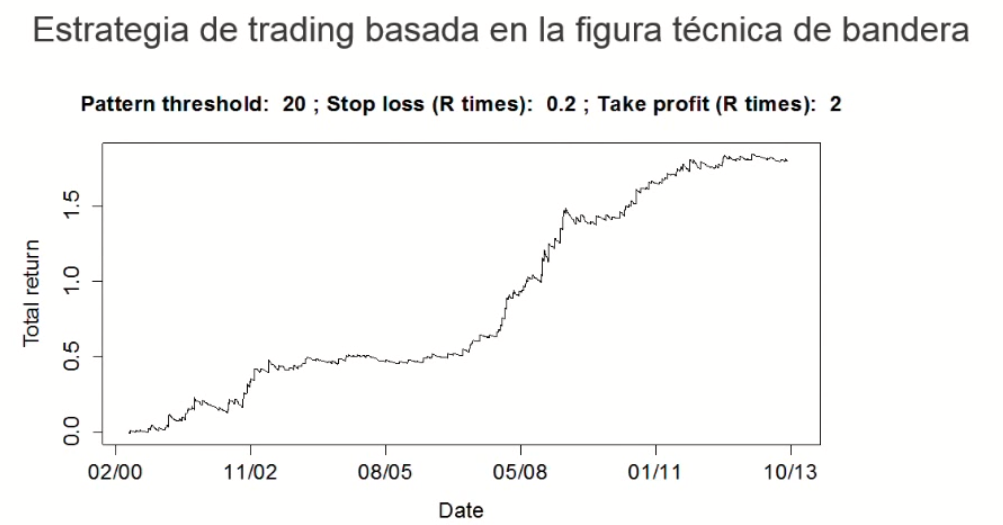
\includegraphics[scale=.65]{images/mod03-16.png}
    \end{center}
    vemos que la estrategia sigue siendo rentable, además es la mejor de las configuraciones, donde el \ti{stop loss = 0.2} y el \ti{take profit = 2}, con una rentabilidad cercana al 200\%, y el drawdown representa un porcentaje realmente pequeño, no va más allá de un 10 al 15 por ciento frente al casi 200 por cien de la rentabilidad.
\end{enumerate}

Podemos comparar esta estragia con una estrategia pasiva de gestión pasica, comparar el índice en el año 2000 y venderlo en el 2013.
\begin{center}
    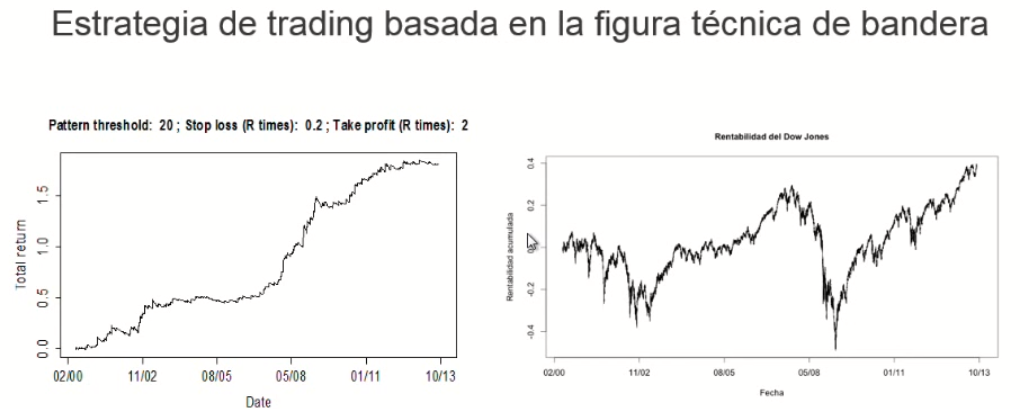
\includegraphics[scale=.65]{images/mod03-17.png}
\end{center}
Si hubieramos realizado esa operación la rentabilidad habría sido del 40\%, habríamos obtenido una rentabilidad inferior a la de la estrategía activa, pero aún más importante el riesgo que estamos asumiendo, \ti{drawdown}, es mucho mayor. En el gráfico de la derecha, vemos como el índice, que aproximadamente es el año 2008, iba ganando un 30\% respecto del 2000, llegó a bajar hasta un -50\%, tenemos un \ti{drawdown} de un 80\%, si al final ganamos un 40\% estamos asumiendo el doble de riesgo que beneficio vamos a obtener.

Esto nos da la idea de que nuestra estrategia de gestión activa es mejor que la correspondiente a la gestión pasiva.

Vamos a estudiar una cuestión muy interesanete, la \tb{correlación entre el stop loss y el take profit y la rentabilidad media y el riesgo medio}.



\section{El análisis fundamental}
